\documentclass[t, screen, aspectratio=43]{beamer}
\usepackage[T1]{fontenc}
\usepackage[utf8]{inputenc}
\usepackage{epsf}
\usepackage{graphicx}
\usepackage{geometry}
\usepackage{tabularx}
\usepackage[table]{colortbl}
% Use the NTNU-temaet for beamer 
% \usetheme[style=ntnu|simple|vertical|horizontal, 
%     language=bm|nn|en, 
%     smalltitle, 
%     city=all|trondheim|alesund|gjovik]{ntnu2017}
\usetheme[style=helvet,language=en]{ntnu2017}

\usepackage[english]{babel}
\usepackage[style=numeric,backend=biber,natbib=false,sorting=none]{biblatex}

\title[Short title]{Ultra-Low Power PLL for Wake-up Receiver Applications}
\subtitle{Specialization Project Progress - 2nd Week}
\author[C Nielsen]{Cole Nielsen}
\institute[NTNU]{Department of Electronic Systems, NTNU}
\date{6 September 2019 (Week 36)}
%\date{} % To have an empty date

\addbibresource{example.bib} % Add bibliography database

% Set the reference style to numeric.
% See here: http://tex.stackexchange.com/questions/68080/beamer-bibliography-icon
\setbeamertemplate{bibliography item}[text] 

% Set bibliography fonts to a small size.
\renewcommand*{\bibfont}{\footnotesize}

\begin{document}

\begin{frame}
\titlepage%
\end{frame}

% Alternatively, special title page command to get a different background
% \ntnutitlepage

% #############################################################################
% This week
% #############################################################################

\begin{frame}
	\frametitle{This Week}
	\begin{block}{Timeline Tasks}
		\begin{itemize}
			\footnotesize
			\item \textbf{Primary:} Review PLL literature/theory to get up to speed on project.
			\begin{itemize}
				\footnotesize
				\item Main topic of interest is design of digital PLLs.
				\begin{itemize}
					\item Decide starting point for modeling based from this.
				\end{itemize} 
				\item Reviewed Texts:	
				\begin{itemize}
					\footnotesize
					\item "Phase Locked Loops: Design, Simulation and Applications", 6th Edition, R.E. Best.
					\item "PLL Performance, Simulation and Design", 5th Edition, D. Banerjee. 
				\end{itemize}
			\end{itemize} 

		\end{itemize}    
	\end{block}
\end{frame}

% #############################################################################
% System modeling
% #############################################################################

\begin{frame}
	\frametitle{System Modeling/Simulation}
	\begin{block}{Initial Approach}
		\vspace{-.2em}
		\begin{itemize}
			\footnotesize
			\item Started writing Python code to simulate digital PLL.
			\begin{itemize}
				\footnotesize
				\item Most familiar for me (I have modelled CDRs in Python before).
				\item Simple to implement digital filters with Python Control Systems Library.
				\begin{itemize}
					\scriptsize
					\item Also - Convenient stability analysis.
				\end{itemize}
			\end{itemize}
			\footnotesize
			\item Decided starting point:
			\begin{itemize}
				\footnotesize
				\item Model DCO based on physical phase-noise limit of ring-oscillators. 
				\item Model loop filter as digital IIR second-order LPF (approximate second-order type-II analog PLL).
				\item Ideal divider and TDC.
			\end{itemize} 
			\item Investigate (to determine component requirements):
			\begin{itemize}
				\footnotesize
				\item Loop-BW to achieve PN requirements. Closed-loop sensitivity analysis:
				\begin{itemize}
					\scriptsize
					\item TDC phase noise significant at f<BW, determine limits for this. 
				\end{itemize}
			\end{itemize}
		\end{itemize}    
	\end{block}
\end{frame}

% continued

\begin{frame}
	\frametitle{System Modeling/Simulation}
	\begin{block}{Initial Approach (continued)}
		\begin{itemize}
			\footnotesize
			\item Investigate (continued):
			\begin{itemize}
				\footnotesize
				\item Quantization, linearity impact of TDC \& DCO on phase noise.
				\begin{itemize}
					\scriptsize
					\item Determine number of bits required for each, and non-linearity limits.  
				\end{itemize}
				\item Loop filter implementations (IIR vs FIR), order \& type.
				\begin{itemize}
					\scriptsize
					\item Evaluate stability, lock time, operating region to meet requirements. 
				\end{itemize}
				\item Digital data path requirements to implement filter.
				\item Algorithm/state machine for handling continuity of fine/coarse DCO ranging. 
				\begin{itemize}
					\scriptsize
					\item Previous two lead to Verilog description.  
				\end{itemize}
			\end{itemize}
			\item \textbf{Final Outcomes:}
			\begin{itemize}
				\footnotesize
				\item Full design constraints for PLL components, sufficient to allow schematic-level implementation.
			\end{itemize}
		\end{itemize}    
	\end{block}
\end{frame}

% continued

\begin{frame}
	\frametitle{System Modeling/Simulation}
	\begin{block}{Implementation in Cadence}
		\vspace{-.2em}
		\begin{itemize}
			\footnotesize
			\item When initial modeling/simulation satisfactory, translate design into a setup within Cadence.
			\begin{itemize}
				\footnotesize
				\item Implement using Verilog-A, ahdlLib components?
			\end{itemize}
			\footnotesize
			\item Will act as known-good test bench for testing transistor-level implementations of components in future design stages.
			\begin{itemize}
				\footnotesize
				\item Replace element by element until fully functioning at transistor level.
			\end{itemize}
		\end{itemize}    
	\end{block}
\end{frame}

% #############################################################################
% Specification
% #############################################################################

\begin{frame}
	\frametitle{Specification (unchanged)}
	\begin{block}{Preliminary Performance Targets}
		\scriptsize
		\begin{table}[h!]
			\centering
			\def\arraystretch{1.5}		
			\setlength\arrayrulewidth{0.75pt}
			\setlength{\tabcolsep}{1em} % for the horizontal padding
			\begin{tabular}{|l|r|l|l|}
				\hline 
				\rule[-1ex]{0pt}{2.5ex} \cellcolor{gray!40}\textbf{Parameter} & \cellcolor{gray!40}\textbf{Value} & \cellcolor{gray!40}\textbf{Unit }& \cellcolor{gray!40}\textbf{Notes}\\ 
				\hline 
				\rule[-1ex]{0pt}{2.5ex} \textbf{Frequency}  & 2.4-2.4835 & GHz & 2.4G ISM Band\\ 
				\hline 
				\rule[-1ex]{0pt}{2.5ex} \textbf{Ref. frequency} & 16 & MHz & Yields 6 channels \\ 
				\hline 
				\rule[-1ex]{0pt}{2.5ex} \textbf{Power} & $\leq$ 100  &$\mu$W & \\ 
				\hline 
				\rule[-1ex]{0pt}{2.5ex} \textbf{Residual FM} & $\leq$ 107  &kHz$_{RMS}$ & BER $\leq$ 1e-2, $f_{dev}$=$\pm$250 KHz\\ 
				\hline 
				\rule[-1ex]{0pt}{2.5ex} \textbf{Initial Lock Time} & $\leq$ 50 & $\mu$s & Upon cold start \\ 
				\hline 
				\rule[-1ex]{0pt}{2.5ex} \textbf{Re-lock Time} & $\leq$ 5 & $\mu$s & Coming out of standby \\ 
				\hline 
				\rule[-1ex]{0pt}{2.5ex} \textbf{Bandwidth} & 100 & kHz & (nominally), tunable \\ 
				\hline 
			\end{tabular} 
			% \caption{Assigned specifications for branch line hybrid design.}
			% \label{asgn_specs}
		\end{table}   
		Additionally: PLL output should support IQ sampling at LO frequency.
	\end{block}    
\end{frame}

% #############################################################################
% Architecture - block diagram
% #############################################################################

\begin{frame}
	\frametitle{Architecture (unchanged)}
	\begin{block}{Block Diagram}
		\center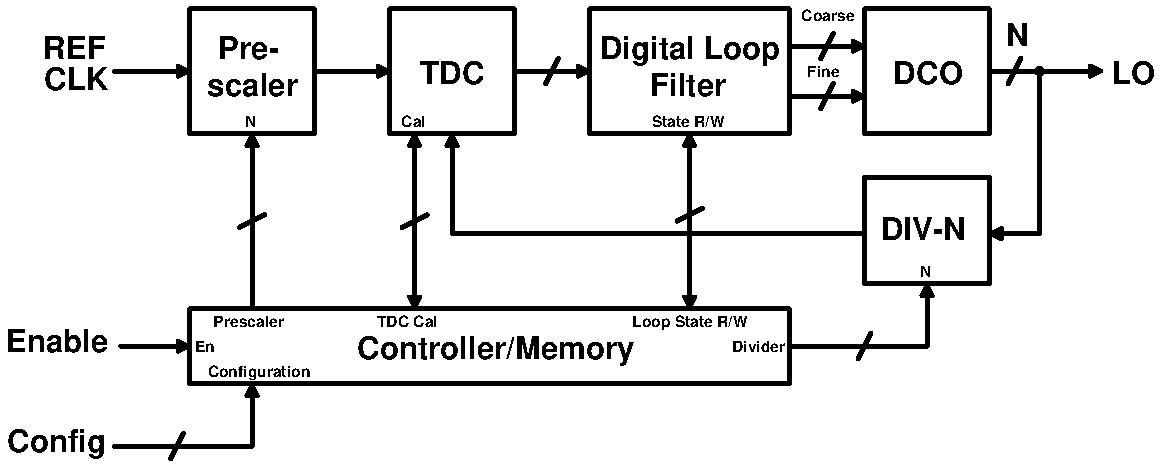
\includegraphics[width=0.75\textwidth, angle=0]{pll2.pdf}

		\end{block}
		\begin{block}{Power Targets}
		\vspace{-.1em}
		\begin{table}[htb!]
			\tiny
			\centering
			\def\arraystretch{1.5}		
			\setlength\arrayrulewidth{0.75pt}
			\setlength{\tabcolsep}{1em} % for the horizontal padding
			\begin{tabular}{|l|l|l|l|l|}
				\hline 
				\rule[-1ex]{0pt}{2.5ex} \cellcolor{gray!40}\textbf{DCO} & \cellcolor{gray!40}\textbf{TDC} & \cellcolor{gray!40}\textbf{Divider }& \cellcolor{gray!40}\textbf{Other} & \cellcolor{gray!40}\textbf{SUM} \\ 
				\hline 
				\rule[-1ex]{0pt}{2.5ex} 70 $\mu$W& 20 $\mu$W & 10 $\mu$W & $<<$ 1 $\mu$W & 100 $\mu$W\\ 
				\hline 
			\end{tabular} 
			% \caption{Assigned specifications for branch line hybrid design.}
			% \label{asgn_specs}
		\end{table}   
	\end{block}

\end{frame}

% #############################################################################
% Project phases slide 1
% #############################################################################
\begin{frame}
	\frametitle{Autumn Timeline}
	\begin{table}[htb!]
		\tiny
		\centering
		\def\arraystretch{1.5}		
		\setlength\arrayrulewidth{0.75pt}
		\setlength{\tabcolsep}{1em} % for the horizontal padding
		\begin{tabular}{|l|l|l|l|}
			\hline 
			\rule[-1ex]{0pt}{2.5ex} \cellcolor{gray!40}\textbf{Week Number} & \cellcolor{gray!40}\textbf{Dates} &\cellcolor{gray!40}\textbf{Tasks} & \cellcolor{gray!40}\textbf{Outcomes}\\ 
			\hline 
			\rule[-1ex]{0pt}{2.5ex} \cellcolor{red!20}\textbf{36}& \cellcolor{red!20}2.9 - 8.9 & \cellcolor{red!20}Review PLL Design & \cellcolor{red!20}Refreshed Knowledge\\ 
			\hline 
			\rule[-1ex]{0pt}{2.5ex} \textbf{37}& 9.9 - 15.9 & Modeling/simulation (set up) & --\\ 
			\hline 
			\rule[-1ex]{0pt}{2.5ex} \textbf{38}& 16.9 - 22.9 & Modeling/simulation & TDC/DCO Requirements\\ 
			\hline 
			\rule[-1ex]{0pt}{2.5ex} \textbf{39}& 23.9 - 29.9& Modeling/simulation& Loop Filter/Digital Algorithms\\ 
			\hline 
			\rule[-1ex]{0pt}{2.5ex} \textbf{40}& 30.9 - 6.10& Modeling/simulation& Ideal (ahdlLib?) implementation in Cadence of PLL\\ 
			\hline 
			\rule[-1ex]{0pt}{2.5ex} \textbf{41}& 7.10 - 13.10& Circuit Research & DCO/Divider topologies\\ 
			\hline 
			\rule[-1ex]{0pt}{2.5ex} \textbf{42}& 14.10 - 20.10& Circuit Research & TDC/other topologies\\ 
			\hline 
			\rule[-1ex]{0pt}{2.5ex} \textbf{43}& 21.10 - 27.10& Circuit Implementation& Digital logic (schematic)\\ 
			\hline 
			\rule[-1ex]{0pt}{2.5ex} \textbf{44}& 28.10 - 3.11& Circuit Implementation& DCO (schematic)\\ 
			\hline 
			\rule[-1ex]{0pt}{2.5ex} \textbf{45}& 4.11 - 10.11& Circuit Implementation& Divider/other (schematic)\\ 
			\hline 
			\rule[-1ex]{0pt}{2.5ex} \textbf{46}& 11.11 - 17.11& Circuit Implementation (TDC)& \\ 
			\hline 
			\rule[-1ex]{0pt}{2.5ex} \textbf{47}& 18.11 - 24.11& Circuit Implementation (TDC)& TDC (schematic)\\ 
			\hline 
			\rule[-1ex]{0pt}{2.5ex} \textbf{48}& 25.11 - 1.12& Full Circuit testing & Testbenches, find bugs, design fixes\\ 
			\hline 
			\rule[-1ex]{0pt}{2.5ex} \textbf{49}& 2.12 - 8.12& Full Circuit testing& Design Fixes/iteration\\ 
			\hline 
			\rule[-1ex]{0pt}{2.5ex} \textbf{50}& 9.12 - 15.12& --& --\\ 
			\hline 
		\end{tabular}
		\begin{flushleft}*I will write the report simultaneously with the work.
		\end{flushleft}
		% \caption{Assigned specifications for branch line hybrid design.}
		% \label{asgn_specs}
	\end{table}   
\end{frame}

% #############################################################################
% Project phases
% #############################################################################

\begin{frame}
	\frametitle{Project Phases}
	\begin{block}{Autumn 2019}
		\footnotesize
		\begin{itemize}
			\item System modeling and simulation.
			\begin{itemize}
				\footnotesize
				\item Learn PLL theory in detail
				\item Evaluate feasability of PLL architectures (counter, TDC-based)
				\item Determine requirements for TDC/DCO/Divider/logic (bits of resolution, accuracy etc) to meet PLL performance specifications.
				\item Determine digital logic for loop filter, validate stability and lock time performance.
			\end{itemize}
			\item Research ultra-low power circuit topologies to implement system components that will meet determined requirements.
			\item Translate component-level specifications into schematic-level circuit designs.
			\begin{itemize}
				\footnotesize
				\item Try, fail, try again until functional at schematic level.
				\begin{itemize}
					\footnotesize
					\item I expect the TDC to be difficult.
				\end{itemize}
			\end{itemize}      
		\end{itemize}
	\end{block}
\end{frame}

% Project phases slide 2

\begin{frame}
	\frametitle{Project Phases (continued)}
	\begin{block}{Spring 2020}
		\begin{itemize}
			\footnotesize
			\item Finalize schematic-level design.
			\item Estabilish thorough tests for PLL performance (automated?) to help in layout.
			\item Layout of PLL.
			\begin{itemize}
				\footnotesize
				\item Design iteration until design specs met.
				\item Probably very time consuming.
			\end{itemize}
			\item Full characterization/validation of design performance. 
			\begin{itemize}
				\footnotesize
				\item Comprehensive Corners/Monte-Carlo testing (time consuming??)
				\item More design iteration if new issues crop up...
			\end{itemize}
			\item Thesis paper writing.
		\end{itemize}
	\end{block}
\end{frame}



\end{document}
